\begin{figure*}[!t]
    \centering
  \begin{minipage}{.49\textwidth}
        \captionsetup{labelsep=space,justification=centering}
        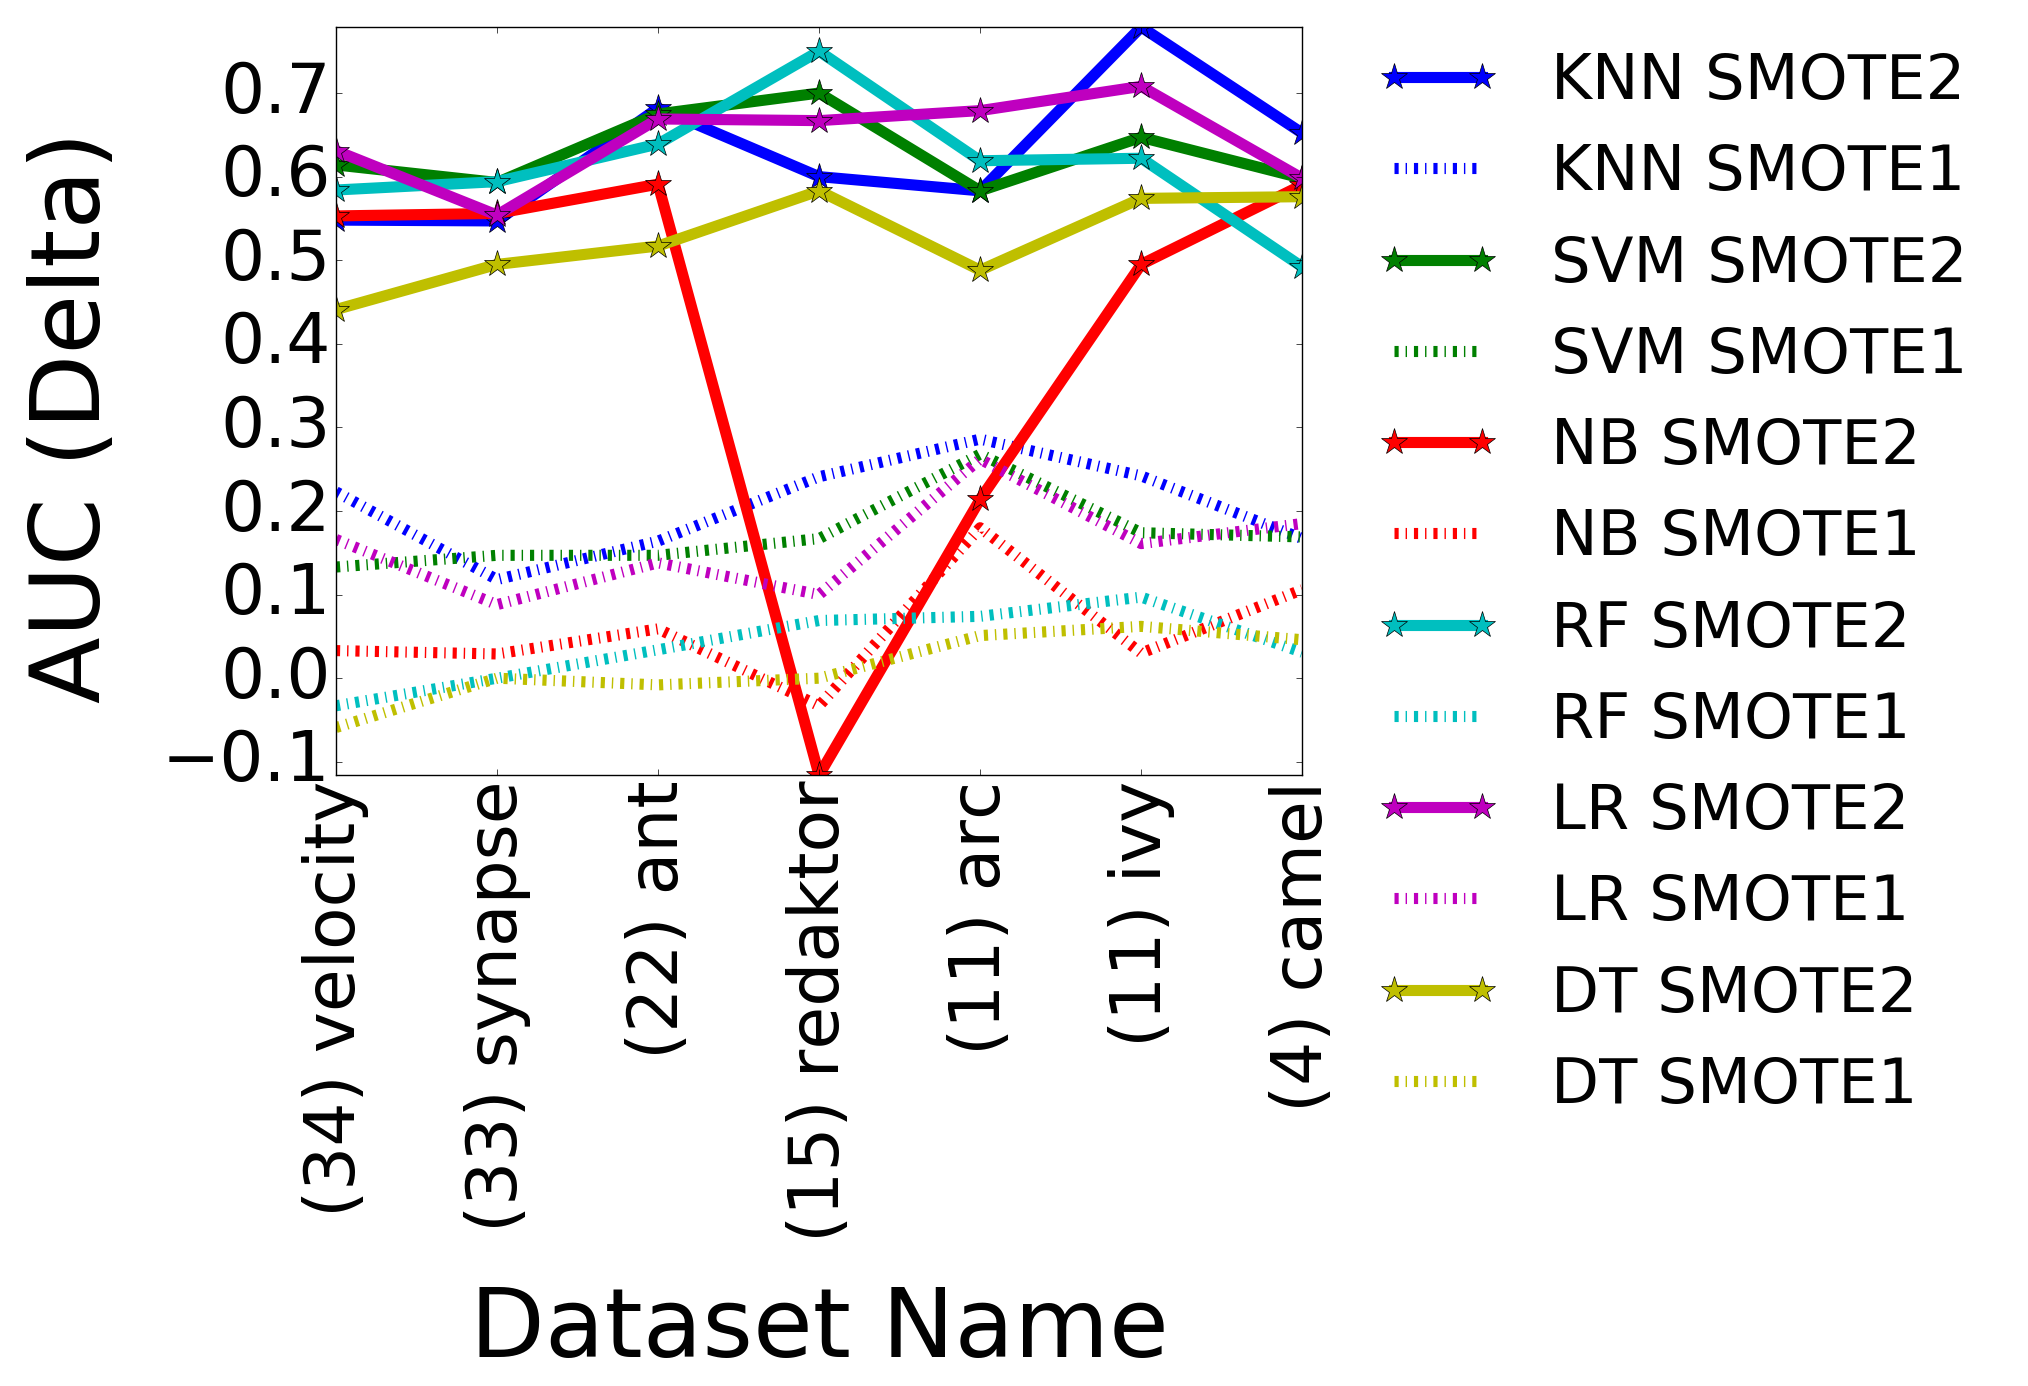
\includegraphics[width=\linewidth]{./fig/AUC_tuned2.png}
  \caption{Area Under Curve}
  \label{AUC}
  \end{minipage}
  \begin{minipage}{.49\textwidth}
        \captionsetup{justification=centering}
        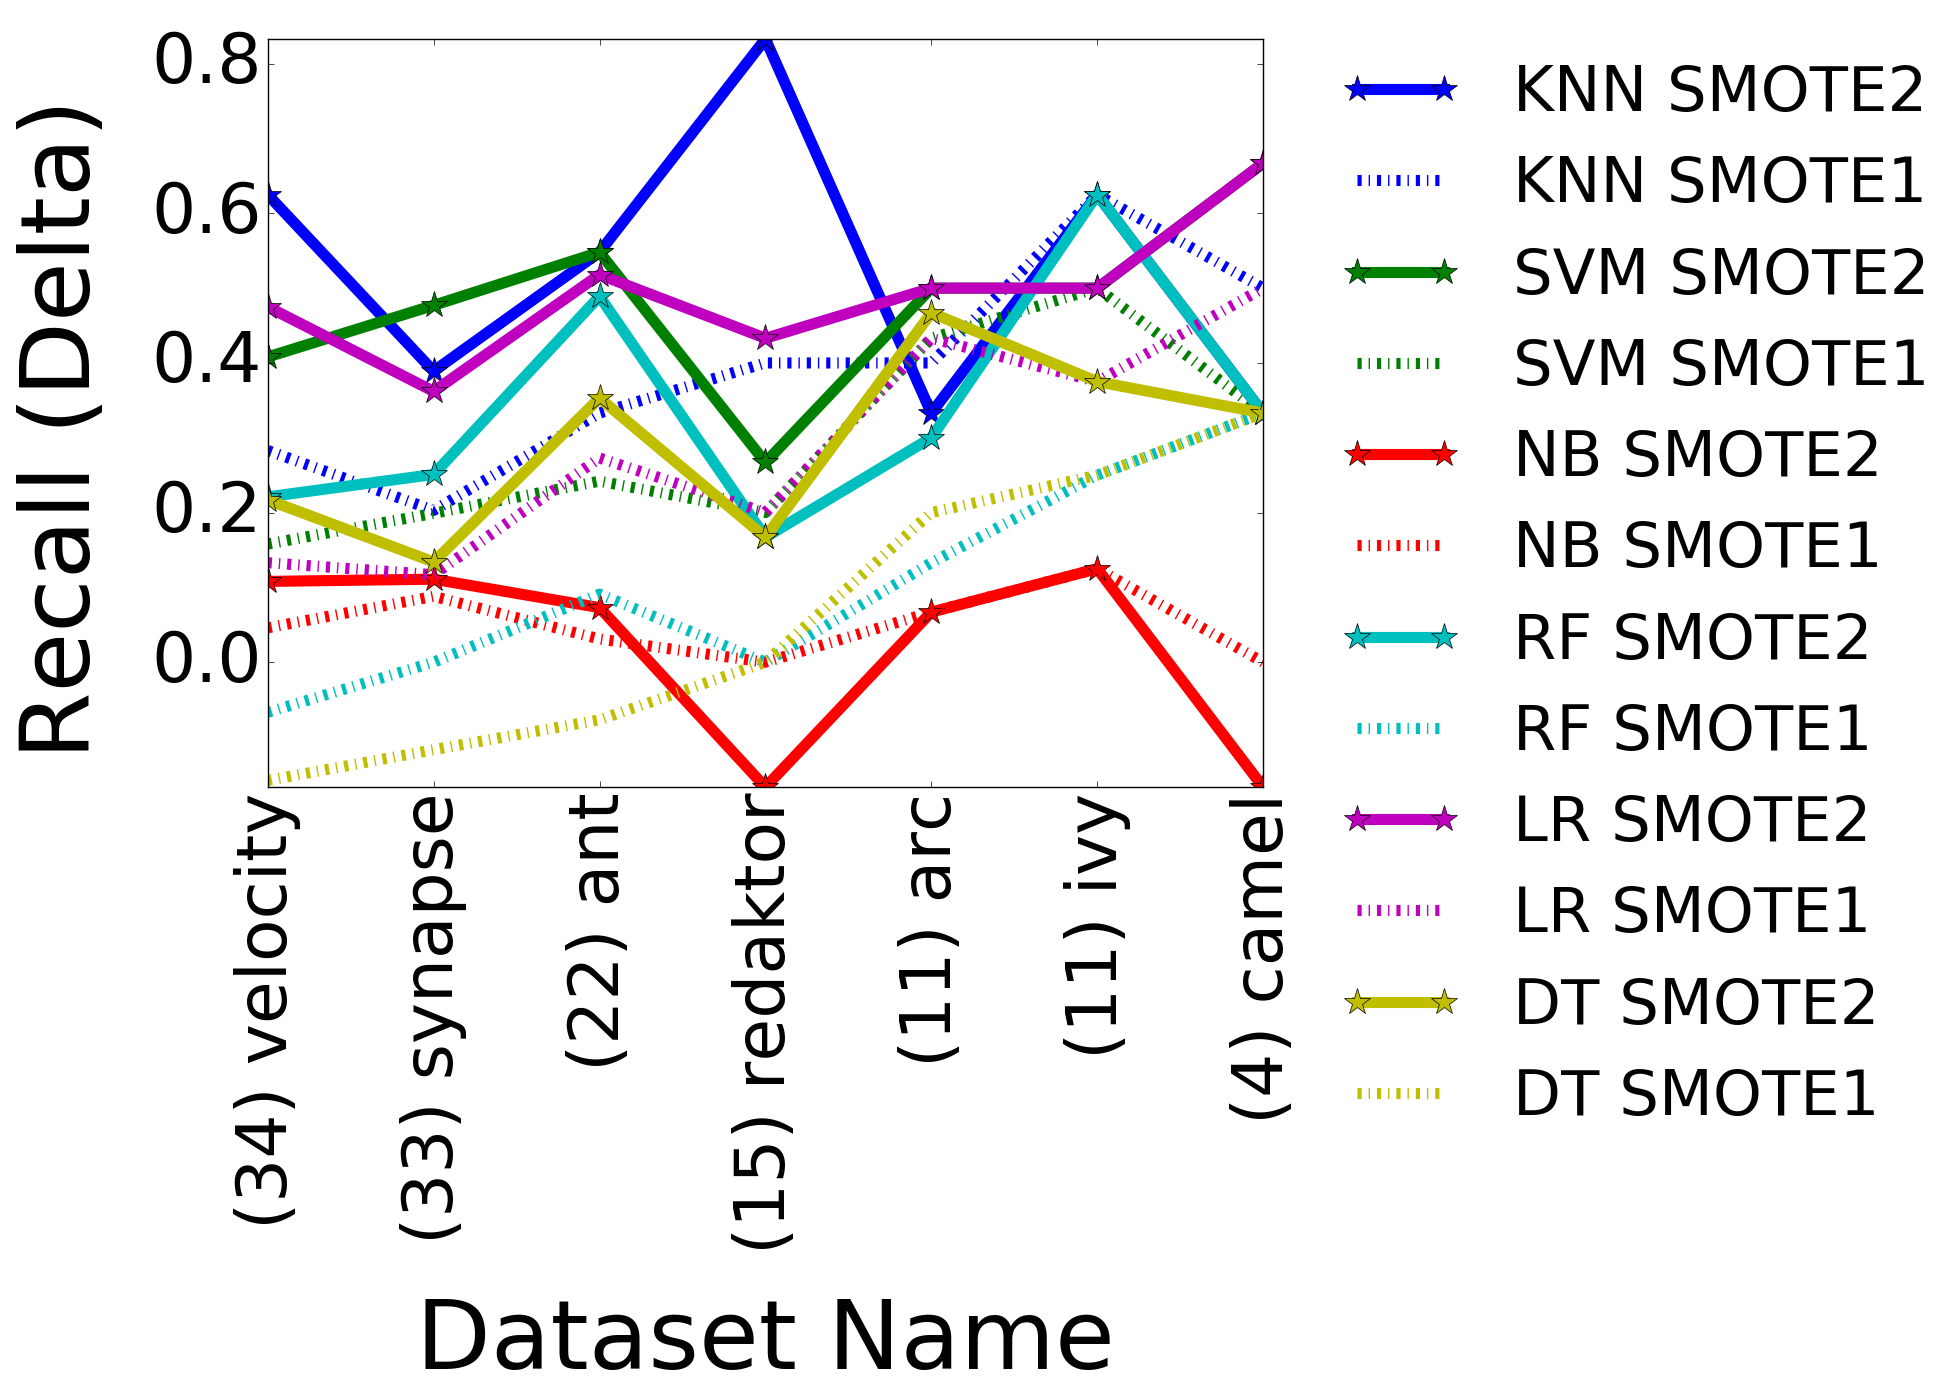
\includegraphics[width=\linewidth]{./fig/Recall_tuned2.png}
  \caption{Recall Scores}
  \label{Recall}
    \end{minipage}%

\end{figure*}

\begin{figure*}[!htbp]
    \centering
      \begin{minipage}{.49\textwidth}
        \captionsetup{justification=centering}
        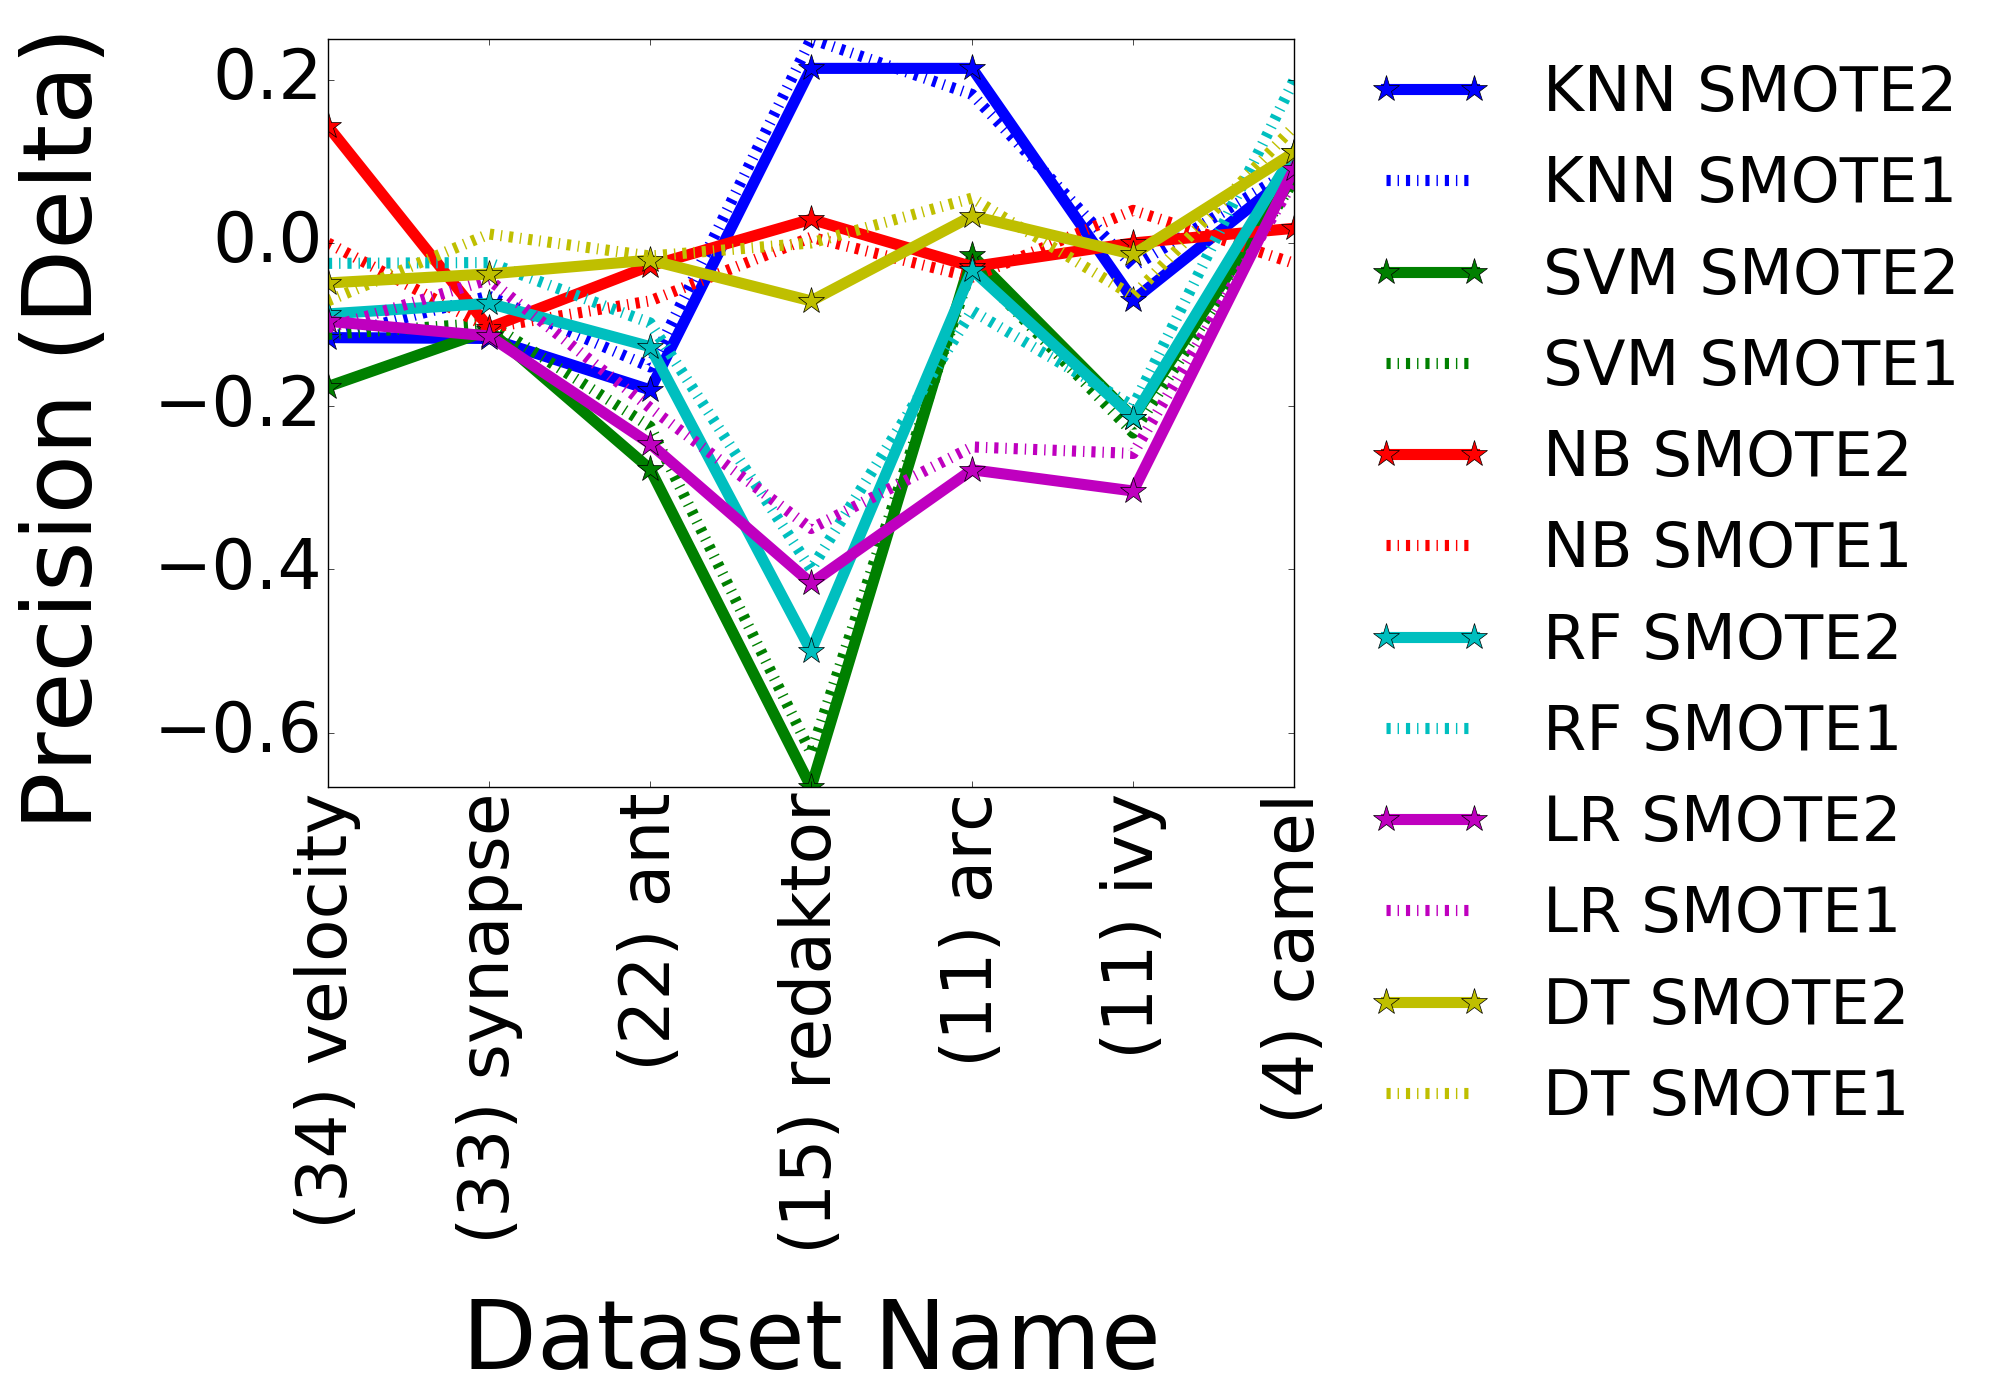
\includegraphics[width=\linewidth]{./fig/Precision_tuned2.png}
  \caption{Precision Scores}
  \label{Precision}
    \end{minipage}%    
  \begin{minipage}{.49\textwidth}
        \captionsetup{justification=centering}
        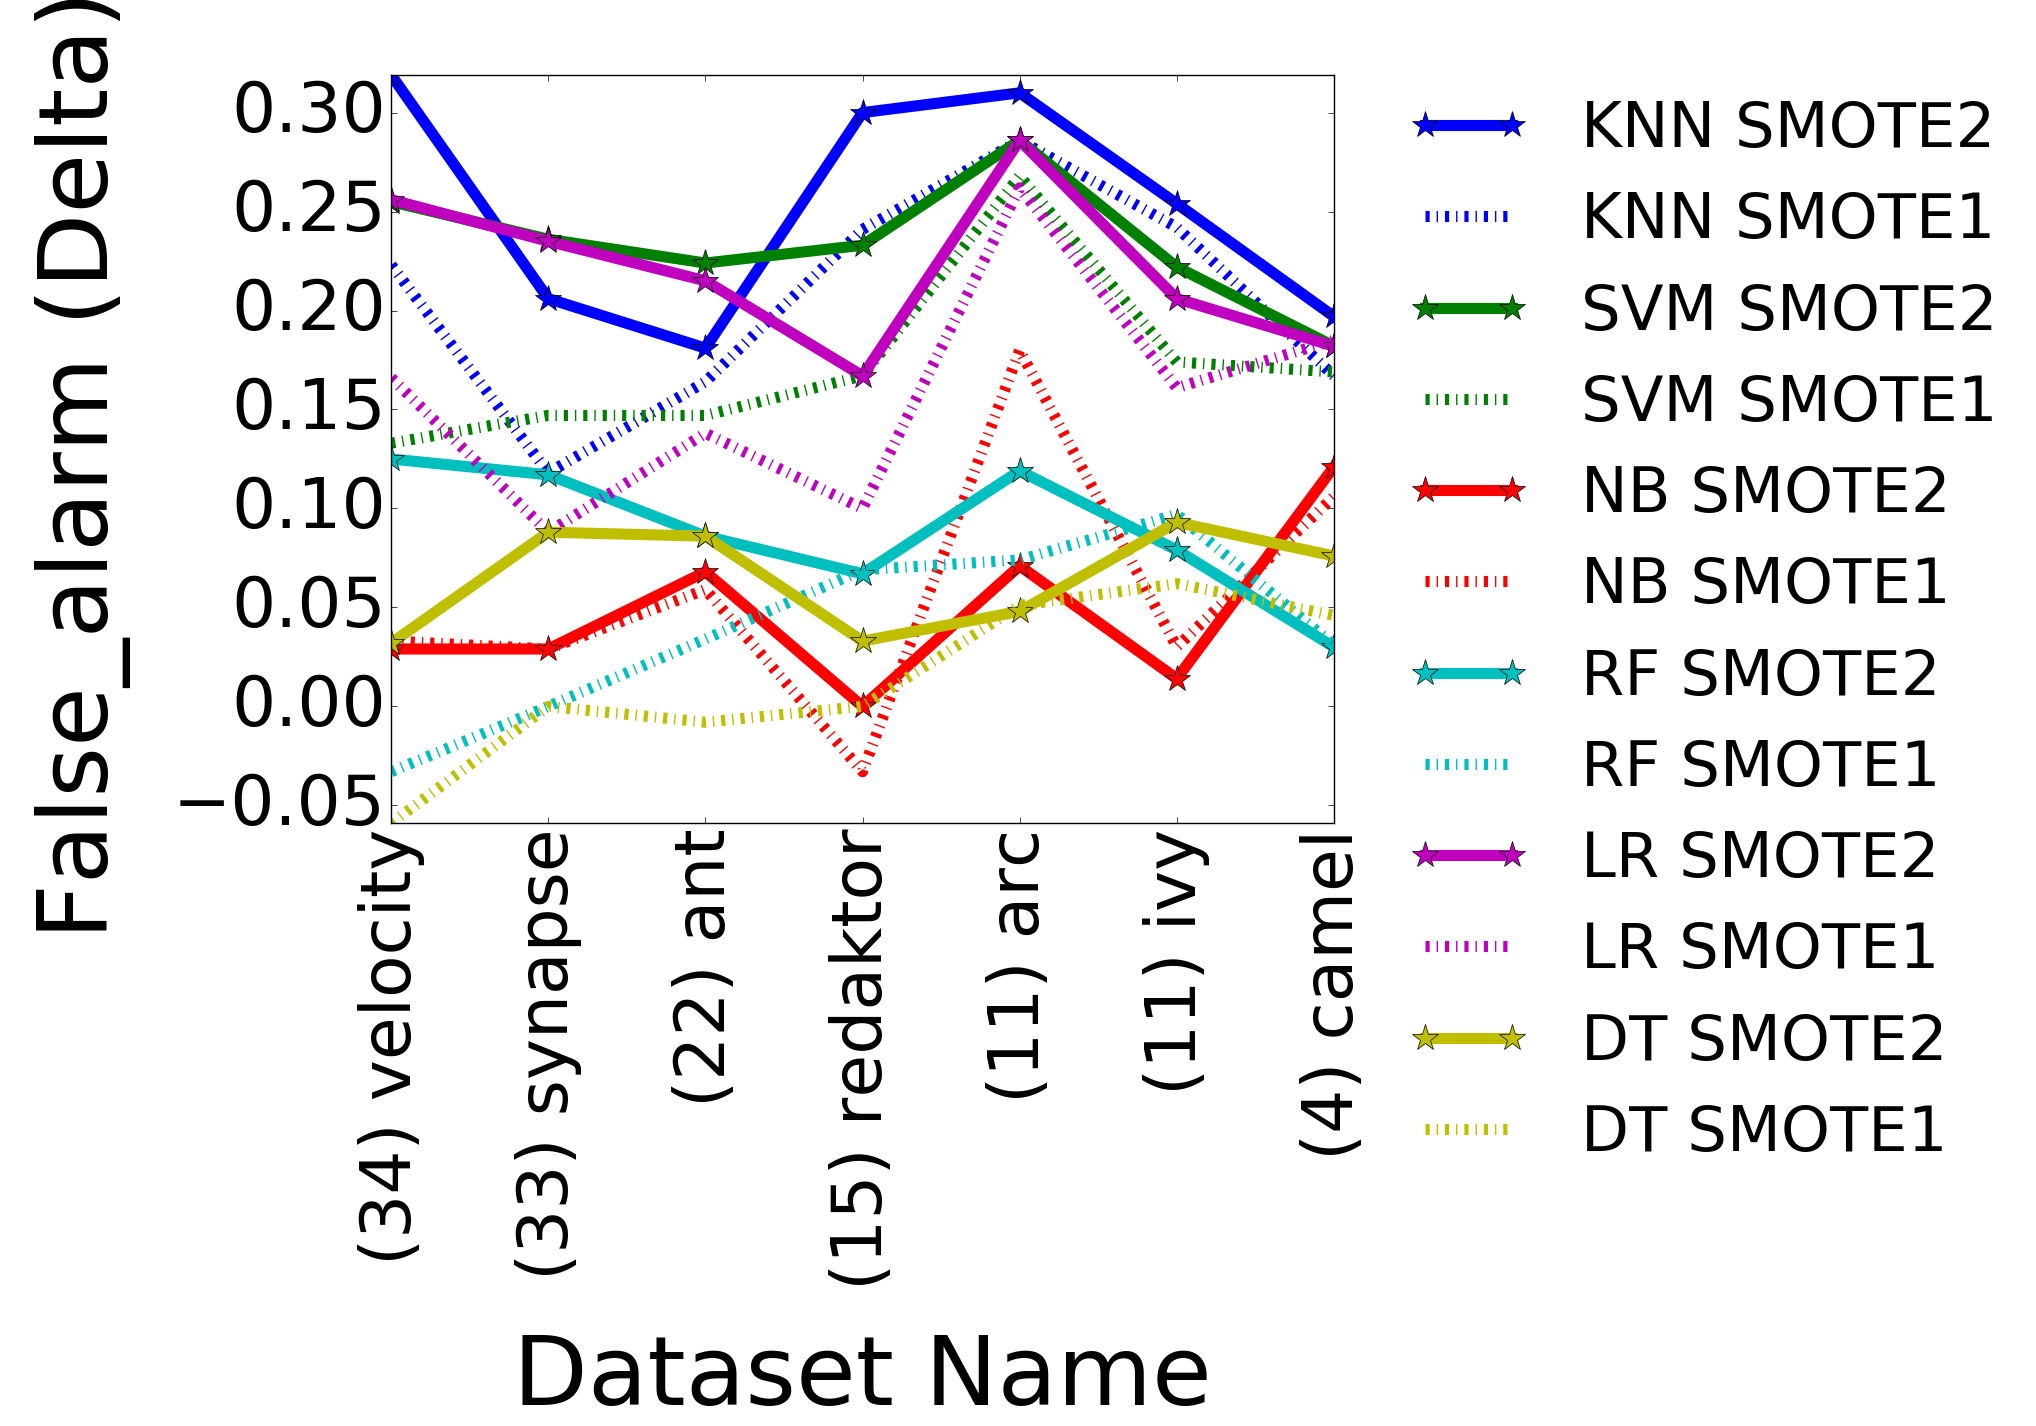
\includegraphics[width=\linewidth]{./fig/False_alarm_tuned2.png}
  \caption{False Alarm Scores}
  \label{false}
    \end{minipage}%
\end{figure*}

\section{Results}
\label{sect:results}
Figures ~\ref{AUC},~\ref{Recall},~\ref{Precision} and~\ref{false} represents all the 4 evaluation criteria against the 6 learners. X-axis represents all 7 datasets in the decreasing percentage of defective classes from left to right. The corresponding percentage is written beside each dataset. Y-axis represents absolute delta improvement between 2 results. Dashed lines represent absolute delta improvement between SMOTE1 - No SMOTE results. Solid lines represent absolute delta improvement between SMOTE2 - No SMOTE results. For figures ~\ref{AUC},~\ref{Recall},~\ref{Precision}, more positive the better and if negative then worse. But for figure ~\ref{false}, it is the other way around. Negative represents better and more positive shows worse results.

\subsection{\textbf{RQ1: Is standard ``off-the-shelf'' SMOTE1 with their default tunings recommended for defect prediction?}}

From all the 4 figures mentioned above, we are seeing about 25\% improvement in AUC for 3 learners which are KNN, LR and SVM (Figure~\ref{AUC}). For other learners the improvements are either 0 or becomes negative by 5\%. It is recommended to use SMOTE1 for these 3 learners. For recall, doing SMOTE1 is highly recommended for imbalanced datasets. All 6 learners kept performing better and better as defective class percentage went minor and minor (Figure~\ref{Recall}). This is what was expected for applying SMOTE.

In terms of precision (Figure~\ref{Precision}), we are seeing a decreasing performance for most datasets against most learners. This concludes we shouldn't be using SMOTE1 if the goal is to have better precision. If we used SMOTE, then it comes with an expense of increasing false alarm (Figure~\ref{false}).

\begin{lesson}
    For defect data, SMOTE1 has little effect on 
 precision, modest improvements for AUC(pf,recall) and largest improvements for recall.
\end{lesson}

\subsection{\textbf{RQ2: Is tuned SMOTE better than the standard untuned SMOTE?}}

From all the 4 figures mentioned above, we are seeing minimum of 50\% improvement than SMOTE1 for AUC for all 6 learners (Figure~\ref{AUC}). It is highly recommended to use SMOTE2 if the tuning goal is to improve higher AUC. For recall, doing SMOTE2 has good improvements than SMOTE1. And all 6 learners kept performing better and better as defective class percentage went minor and minor (Figure~\ref{Recall}). This is what was expected for applying SMOTE.

In terms of precision (Figure~\ref{Precision}), we are seeing a decreasing performance for most datasets against most learners which is similar to what was observed with SMOTE1 results. This concludes we shouldn't be using SMOTE2 if the goal is to have better precision. And if we used SMOTE2, then it comes with some not large false alarm increase (Figure~\ref{false}).

\begin{lesson}
    For defect data, SMOTE2  
 offers   large  improvements over SMOTE1 for recall
 and dramatic improvements for AUC (pf,recall).
\end{lesson}

\subsection{\textbf{RQ3: Do different data sets
      need different configurations with SMOTE2?}}

abc

\begin{lesson}
    DE finds different ``best'' parameter settings for SMOTE for different data sets. Hence reusing tunings  suggested  by  any other  previous study  for any dataset is \underline{{\em not}} recommended. Instead,  it is better to
      use  automatic  tuning  methods  to find the best tuning parameters for the current data set.
\end{lesson}

\begin{figure}[!b]
  \captionsetup{justification=centering}
  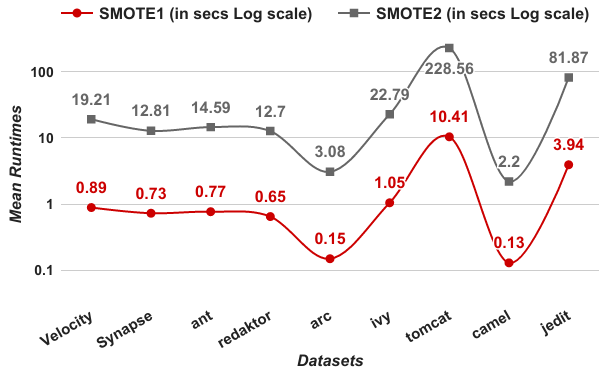
\includegraphics[width=\linewidth]{./fig/runtimes.png}
  \caption{Datasets vs Runtimes}
  \label{runtime}
\end{figure} 

\subsection{\textbf{RQ4: Is tuning extremely slow?}}

Search-based SE methods can be very slow. Wang et al.~\cite{wang2013searching} once needed 15
years of CPU time to find and verify the tunings required for software
clone detectors. Sayyad et al.~\cite{sayyad2013scalable} routinely used
$10^6$ evaluations (or more) of their models in order to extract
products from highly constrained product
lines. Hence, before recommending any
search-based method, it is wise to consider the runtime cost of that
recommendation.

To understand our timing results, recall that SMOTE2 uses
Algorithm~1. Based on the psuedocode
shown above, our pre-experimental expectation is that
tuning will be three times slower than not tuning.
 
Figure~\ref{runtimes} check if that theoretical
holds true in practice. Shown in circle and square markers are the
  runtimes required to run SMOTE1 and SMOTE2 respectively.  The
  longer runtimes (in square) include the times required for DE to find
  the tunings. Overall, tuning slows down LDA by a factor of up to
  five (which is very close to our theoretical prediction).

\begin{lesson}
    Tuning with DE makes training three to five times slower, but the improvements which we get for AUC and recall is quite advantageous.
\end{lesson}
